\chapter{Intermediate Algebra}

\section{Review and Expanding on Various Topics}

Phuong trình một biến $x$ có thể có: một nghiệm, vô nghiệm hoặc vô số nghiệm.

\section{Systems of Equations}

% \vspace{1 cm}
%
% \centerline{\textbf{\large System of Equations with No Solution or Infinite Solutions}}
%
% \vspace{0.2 cm}

System of Equations can have: một cặp nghiệm (x,y), no Solution or Infinite Solutions.

There are three methods for solving systems of Equations:

\begin{enumerate}
  \item Substitution: lấy 1 phương trình dễ tìm x theo y, sau đó thay x vừa tìm vào phương trình còn lại tìm y.
  \item Elimination: cộng hoặc trừ 2 phương trình lại với nhau để khử đi một biến
  \item Graphing
\end{enumerate}

Only Substitution \& Elimination được dùng in the real world. Graphing is really not practical, takes too long, not reliable.

% \begin{equation}
%   \begin{cases}
%     x+4y = 5\\
%     x-4y=-3
%   \end{cases} \iff
%   \begin{cases}
%     x+4y = 5\\
%     x-4y=-3
%   \end{cases} \iff
% \end{equation}

Example of Solving by Elimination (Addition or Subtraction)

% `\right.` is a "phantom" right delimiter
\[
  \begin{aligned}
    &\left\{\begin{aligned} 
      x + 4y &= 5 \\ 
      x - 4y &= -3
    \end{aligned}\right. \iff 
    \left\{\begin{aligned}
      &x +4y = 5\\ 
      &2x = 2
    \end{aligned}\right.
    \\
    \iff &\left\{\begin{aligned} 
      x &= 1 \\ 
      y &= 1
    \end{aligned}\right.
  \end{aligned}
\]

\newpage

Phương pháp elimination, đôi khi phải multiply both equation.

\begin{figure}[htb!]
  \centering
  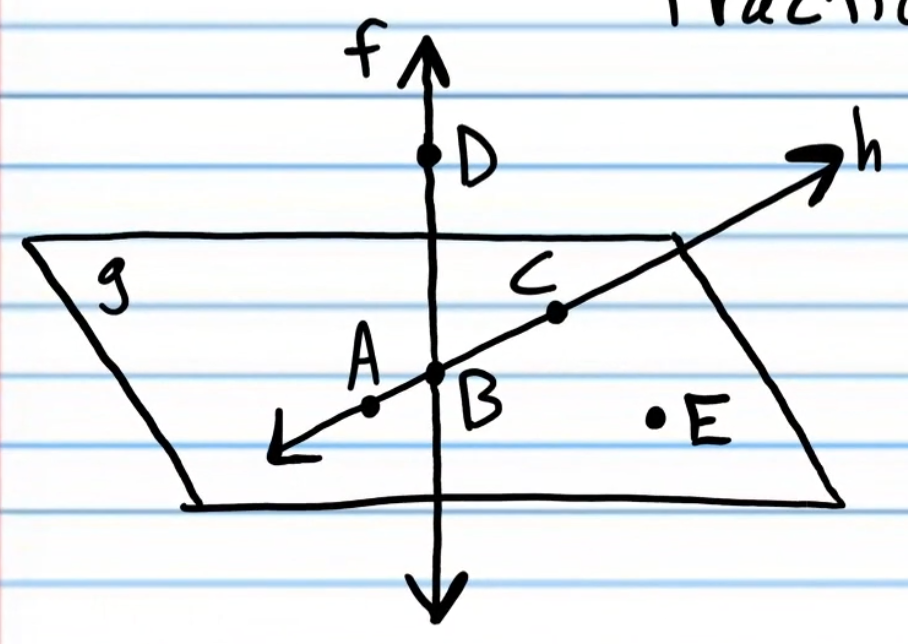
\includegraphics[width=0.5\textwidth]{0201.png}
  \caption{bài tập}
\end{figure}

\section{Linear Equations}

There are three forms of Linear Equations

% \begin{figure}[htb!]
%   \centering
%   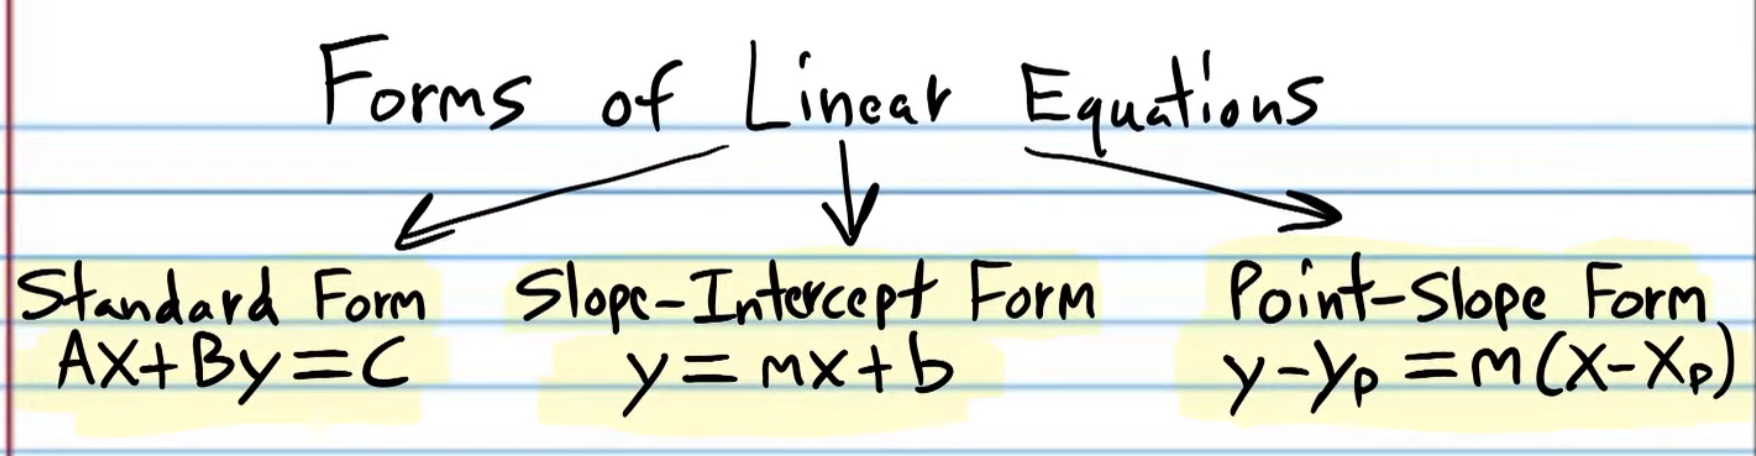
\includegraphics[width=0.7\textwidth]{0202.png}
%   \caption{Forms of Linear Equations}
% \end{figure}

